% Created by tikzDevice version 0.8.1 on 2016-01-23 06:21:33
% !TEX encoding = UTF-8 Unicode
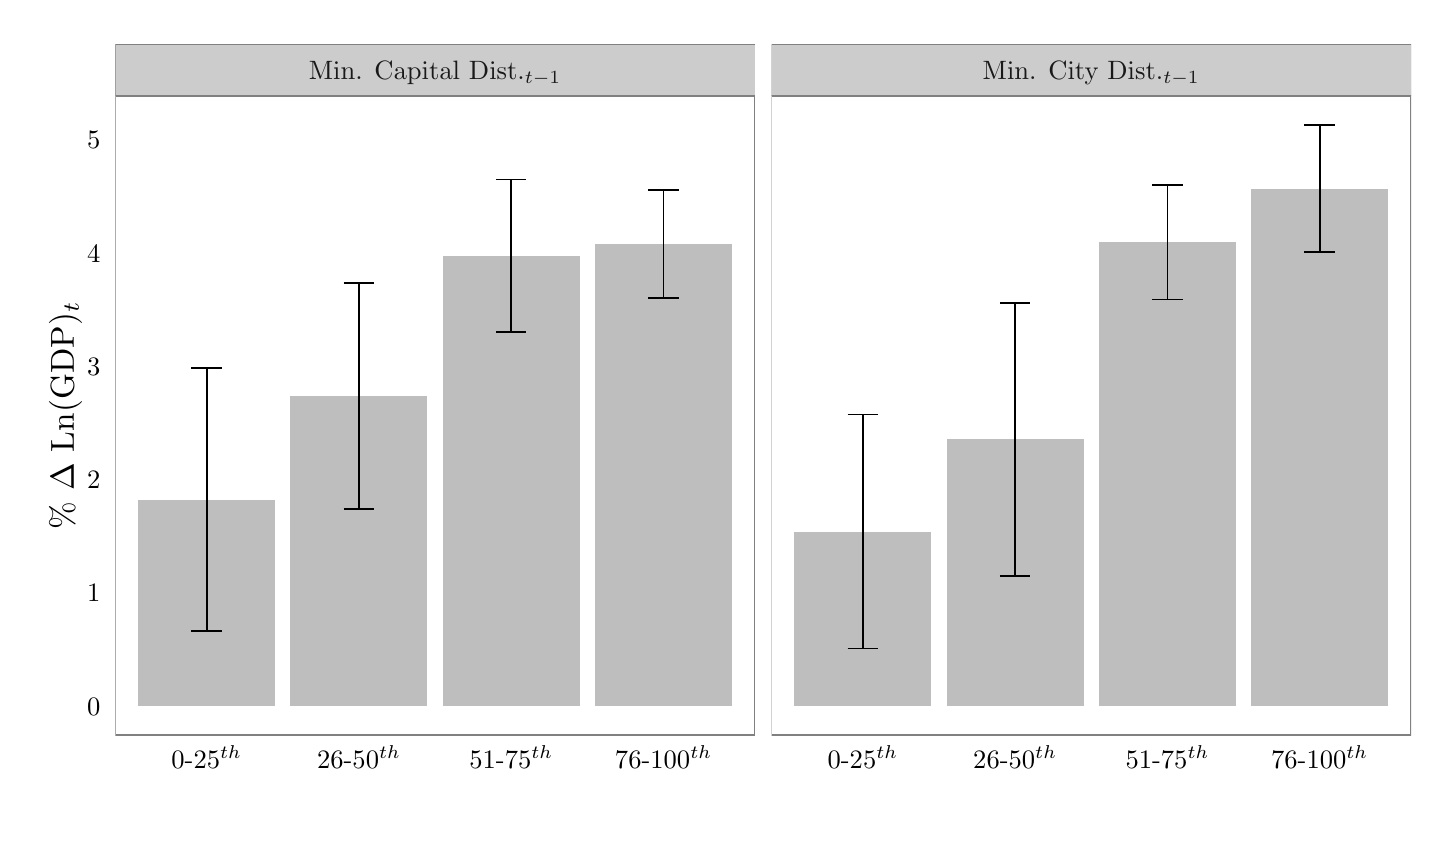
\begin{tikzpicture}[x=1pt,y=1pt]
\definecolor{fillColor}{RGB}{255,255,255}
\path[use as bounding box,fill=fillColor,fill opacity=0.00] (0,0) rectangle (505.89,289.08);
\begin{scope}
\path[clip] (  0.00,  0.00) rectangle (505.89,289.08);
\definecolor{drawColor}{RGB}{255,255,255}
\definecolor{fillColor}{RGB}{255,255,255}

\path[draw=drawColor,line width= 0.6pt,line join=round,line cap=round,fill=fillColor] (  0.00,  0.00) rectangle (505.89,289.08);
\end{scope}
\begin{scope}
\path[clip] ( 31.66, 33.48) rectangle (262.78,264.47);
\definecolor{fillColor}{RGB}{255,255,255}

\path[fill=fillColor] ( 31.66, 33.48) rectangle (262.78,264.47);
\definecolor{fillColor}{RGB}{190,190,190}

\path[fill=fillColor] ( 39.92, 43.98) rectangle ( 89.44,118.52);

\path[fill=fillColor] ( 94.94, 43.98) rectangle (144.47,156.08);

\path[fill=fillColor] (149.97, 43.98) rectangle (199.50,206.62);

\path[fill=fillColor] (205.00, 43.98) rectangle (254.52,210.92);
\definecolor{drawColor}{RGB}{0,0,0}

\path[draw=drawColor,line width= 0.6pt,line join=round] ( 59.18,166.05) --
	( 70.18,166.05);

\path[draw=drawColor,line width= 0.6pt,line join=round] ( 64.68,166.05) --
	( 64.68, 70.99);

\path[draw=drawColor,line width= 0.6pt,line join=round] ( 59.18, 70.99) --
	( 70.18, 70.99);

\path[draw=drawColor,line width= 0.6pt,line join=round] (114.20,196.90) --
	(125.21,196.90);

\path[draw=drawColor,line width= 0.6pt,line join=round] (119.71,196.90) --
	(119.71,115.25);

\path[draw=drawColor,line width= 0.6pt,line join=round] (114.20,115.25) --
	(125.21,115.25);

\path[draw=drawColor,line width= 0.6pt,line join=round] (169.23,234.20) --
	(180.24,234.20);

\path[draw=drawColor,line width= 0.6pt,line join=round] (174.73,234.20) --
	(174.73,179.04);

\path[draw=drawColor,line width= 0.6pt,line join=round] (169.23,179.04) --
	(180.24,179.04);

\path[draw=drawColor,line width= 0.6pt,line join=round] (224.26,230.50) --
	(235.26,230.50);

\path[draw=drawColor,line width= 0.6pt,line join=round] (229.76,230.50) --
	(229.76,191.33);

\path[draw=drawColor,line width= 0.6pt,line join=round] (224.26,191.33) --
	(235.26,191.33);
\definecolor{drawColor}{gray}{0.50}

\path[draw=drawColor,line width= 0.6pt,line join=round,line cap=round] ( 31.66, 33.48) rectangle (262.78,264.47);
\end{scope}
\begin{scope}
\path[clip] (268.78, 33.48) rectangle (499.89,264.47);
\definecolor{fillColor}{RGB}{255,255,255}

\path[fill=fillColor] (268.78, 33.48) rectangle (499.89,264.47);
\definecolor{fillColor}{RGB}{190,190,190}

\path[fill=fillColor] (277.03, 43.98) rectangle (326.56,107.02);

\path[fill=fillColor] (332.06, 43.98) rectangle (381.58,140.28);

\path[fill=fillColor] (387.08, 43.98) rectangle (436.61,211.59);

\path[fill=fillColor] (442.11, 43.98) rectangle (491.64,230.95);
\definecolor{drawColor}{RGB}{0,0,0}

\path[draw=drawColor,line width= 0.6pt,line join=round] (296.29,149.26) --
	(307.30,149.26);

\path[draw=drawColor,line width= 0.6pt,line join=round] (301.79,149.26) --
	(301.79, 64.78);

\path[draw=drawColor,line width= 0.6pt,line join=round] (296.29, 64.78) --
	(307.30, 64.78);

\path[draw=drawColor,line width= 0.6pt,line join=round] (351.32,189.55) --
	(362.32,189.55);

\path[draw=drawColor,line width= 0.6pt,line join=round] (356.82,189.55) --
	(356.82, 91.00);

\path[draw=drawColor,line width= 0.6pt,line join=round] (351.32, 91.00) --
	(362.32, 91.00);

\path[draw=drawColor,line width= 0.6pt,line join=round] (406.34,232.29) --
	(417.35,232.29);

\path[draw=drawColor,line width= 0.6pt,line join=round] (411.85,232.29) --
	(411.85,190.89);

\path[draw=drawColor,line width= 0.6pt,line join=round] (406.34,190.89) --
	(417.35,190.89);

\path[draw=drawColor,line width= 0.6pt,line join=round] (461.37,253.97) --
	(472.38,253.97);

\path[draw=drawColor,line width= 0.6pt,line join=round] (466.87,253.97) --
	(466.87,207.94);

\path[draw=drawColor,line width= 0.6pt,line join=round] (461.37,207.94) --
	(472.38,207.94);
\definecolor{drawColor}{gray}{0.50}

\path[draw=drawColor,line width= 0.6pt,line join=round,line cap=round] (268.78, 33.48) rectangle (499.89,264.47);
\end{scope}
\begin{scope}
\path[clip] ( 31.66,264.47) rectangle (262.78,283.08);
\definecolor{drawColor}{gray}{0.50}
\definecolor{fillColor}{gray}{0.80}

\path[draw=drawColor,line width= 0.2pt,line join=round,line cap=round,fill=fillColor] ( 31.66,264.47) rectangle (262.78,283.08);
\definecolor{drawColor}{gray}{0.10}

\node[text=drawColor,anchor=base,inner sep=0pt, outer sep=0pt, scale=  0.96] at (147.22,270.47) {Min. Capital Dist.$_{t-1}$};
\end{scope}
\begin{scope}
\path[clip] (268.78,264.47) rectangle (499.89,283.08);
\definecolor{drawColor}{gray}{0.50}
\definecolor{fillColor}{gray}{0.80}

\path[draw=drawColor,line width= 0.2pt,line join=round,line cap=round,fill=fillColor] (268.78,264.47) rectangle (499.89,283.08);
\definecolor{drawColor}{gray}{0.10}

\node[text=drawColor,anchor=base,inner sep=0pt, outer sep=0pt, scale=  0.96] at (384.33,270.47) {Min. City Dist.$_{t-1}$};
\end{scope}
\begin{scope}
\path[clip] (  0.00,  0.00) rectangle (505.89,289.08);
\definecolor{drawColor}{RGB}{0,0,0}

\node[text=drawColor,anchor=base east,inner sep=0pt, outer sep=0pt, scale=  0.96] at ( 26.26, 40.67) {0};

\node[text=drawColor,anchor=base east,inner sep=0pt, outer sep=0pt, scale=  0.96] at ( 26.26, 81.59) {1};

\node[text=drawColor,anchor=base east,inner sep=0pt, outer sep=0pt, scale=  0.96] at ( 26.26,122.51) {2};

\node[text=drawColor,anchor=base east,inner sep=0pt, outer sep=0pt, scale=  0.96] at ( 26.26,163.44) {3};

\node[text=drawColor,anchor=base east,inner sep=0pt, outer sep=0pt, scale=  0.96] at ( 26.26,204.36) {4};

\node[text=drawColor,anchor=base east,inner sep=0pt, outer sep=0pt, scale=  0.96] at ( 26.26,245.28) {5};
\end{scope}
\begin{scope}
\path[clip] (  0.00,  0.00) rectangle (505.89,289.08);
\definecolor{drawColor}{RGB}{0,0,0}

\node[text=drawColor,anchor=base,inner sep=0pt, outer sep=0pt, scale=  0.96] at ( 64.68, 21.46) {0-25$^{th}$};

\node[text=drawColor,anchor=base,inner sep=0pt, outer sep=0pt, scale=  0.96] at (119.71, 21.46) {26-50$^{th}$};

\node[text=drawColor,anchor=base,inner sep=0pt, outer sep=0pt, scale=  0.96] at (174.73, 21.46) {51-75$^{th}$};

\node[text=drawColor,anchor=base,inner sep=0pt, outer sep=0pt, scale=  0.96] at (229.76, 21.46) {76-100$^{th}$};
\end{scope}
\begin{scope}
\path[clip] (  0.00,  0.00) rectangle (505.89,289.08);
\definecolor{drawColor}{RGB}{0,0,0}

\node[text=drawColor,anchor=base,inner sep=0pt, outer sep=0pt, scale=  0.96] at (301.79, 21.46) {0-25$^{th}$};

\node[text=drawColor,anchor=base,inner sep=0pt, outer sep=0pt, scale=  0.96] at (356.82, 21.46) {26-50$^{th}$};

\node[text=drawColor,anchor=base,inner sep=0pt, outer sep=0pt, scale=  0.96] at (411.85, 21.46) {51-75$^{th}$};

\node[text=drawColor,anchor=base,inner sep=0pt, outer sep=0pt, scale=  0.96] at (466.87, 21.46) {76-100$^{th}$};
\end{scope}
\begin{scope}
\path[clip] (  0.00,  0.00) rectangle (505.89,289.08);
\definecolor{drawColor}{RGB}{0,0,0}

\node[text=drawColor,rotate= 90.00,anchor=base,inner sep=0pt, outer sep=0pt, scale=  1.20] at ( 16.66,148.97) {\% $\Delta$ Ln(GDP)$_{t}$};
\end{scope}
\end{tikzpicture}
